%% ~~~~~~~~~~~~~~~~~~~~~~~~~~~~~~~~~~~~~~~~~~~~~~~~~~~~~~~~~~~~~~~~~~ %%
%% template document ~~~~~~~~~~~~~~~~~~~~~~~~~~~~~~~~~~~~~~~~~~~~~~~~ %%
%% includes coverpage, table of contents, sections, & figures ~~~~~~~ %%
%% created 4/15/2022; zhr ~~~~~~~~~~~~~~~~~~~~~~~~~~~~~~~~~~~~~~~~~~~ %%
%% ~~~~~~~~~~~~~~~~~~~~~~~~~~~~~~~~~~~~~~~~~~~~~~~~~~~~~~~~~~~~~~~~~~ %%





%% preamble: load packages / document settings ~~~~~~~~~~~~~~~~~~~~~~ %%
\documentclass[11pt]{article}
\usepackage[dvipsnames]{xcolor}
\usepackage[position=top]{subcaption}
\captionsetup[subfigure]{skip=0pt}
\usepackage{float}
\floatstyle{plaintop}
\restylefloat{table}
\usepackage{graphicx}
\graphicspath{{./figs/}}
\usepackage[export]{adjustbox}
\usepackage{caption}
\usepackage{subcaption}
\usepackage{wrapfig}
\usepackage{setspace} 
\usepackage{ragged2e}
\usepackage{authblk}

\usepackage{enumitem}
%\setlist[enumerate,1]{label=(\arabic*),font=\itshape}

%% biblio information 
%\usepackage[
%sorting=none,
%backend=biber,
%style=numeric,
%url=false,
%eprint=false,
%isbn=false
%]{biblatex}
%\addbibresource{./biblio/references.bib}
%% end biblio 

\usepackage[margin=1in]{geometry}
\usepackage[hypertexnames=false]{hyperref}
\hypersetup{urlbordercolor=blue}
\hypersetup{linktocpage=true}
%% END preamble ~~~~~~~~~~~~~~~~~~~~~~~~~~~~~~~~~~~~~~~~~~~~~~~~~~~~~ %%

%% custom commands ~~~~~~~~~~~~~~~~~~~~~~~~~~~~~~~~~~~~~~~~~~~~~~~~~~ %%
\newcommand{\w}{.5\textwidth} % set figure width 
\newcommand{\h}{.45\textwidth} % set figure height
\newcommand{\pt}{\vspace{-.5em}} % reduce vertical spacing 
\newcommand{\ptt}{\vspace{-.9em}} % reduce vertical spacing 
%% END custom commands ~~~~~~~~~~~~~~~~~~~~~~~~~~~~~~~~~~~~~~~~~~~~~~ %%




%% title page and title information ~~~~~~~~~~~~~~~~~~~~~~~~~~~~~~~~~ %%
\title{
August 2022 progress report to the Port of Seattle on the
\\
Urban Kelp Research Project
\\
}
\author{
\Large{
\textbf{Seattle Aquarium} 
$\vert$ 
\textit{Conservation Programs and Partnerships}
}
\\
\large{
Zachary Randell, Ph.D., Research Scientist
\\
Megan Williams, M.S., Research Technician

Shawn Larson, Ph.D., Senior Conservation Research Manager
\\
Erin Meyer, Ph.D., Director
}
\\
\vspace{10pt}
} 


%\textit{\textbf{
%Conservation Programs \& Partnerships, Seattle 
%Aquarium
%}}
\begin{document}
\begin{titlepage}
\maketitle
\tableofcontents
%\thispagestyle{empty}
%\tableofcontents
\vfill
%\centering
%\begin{figure}[h!]
%\centering
%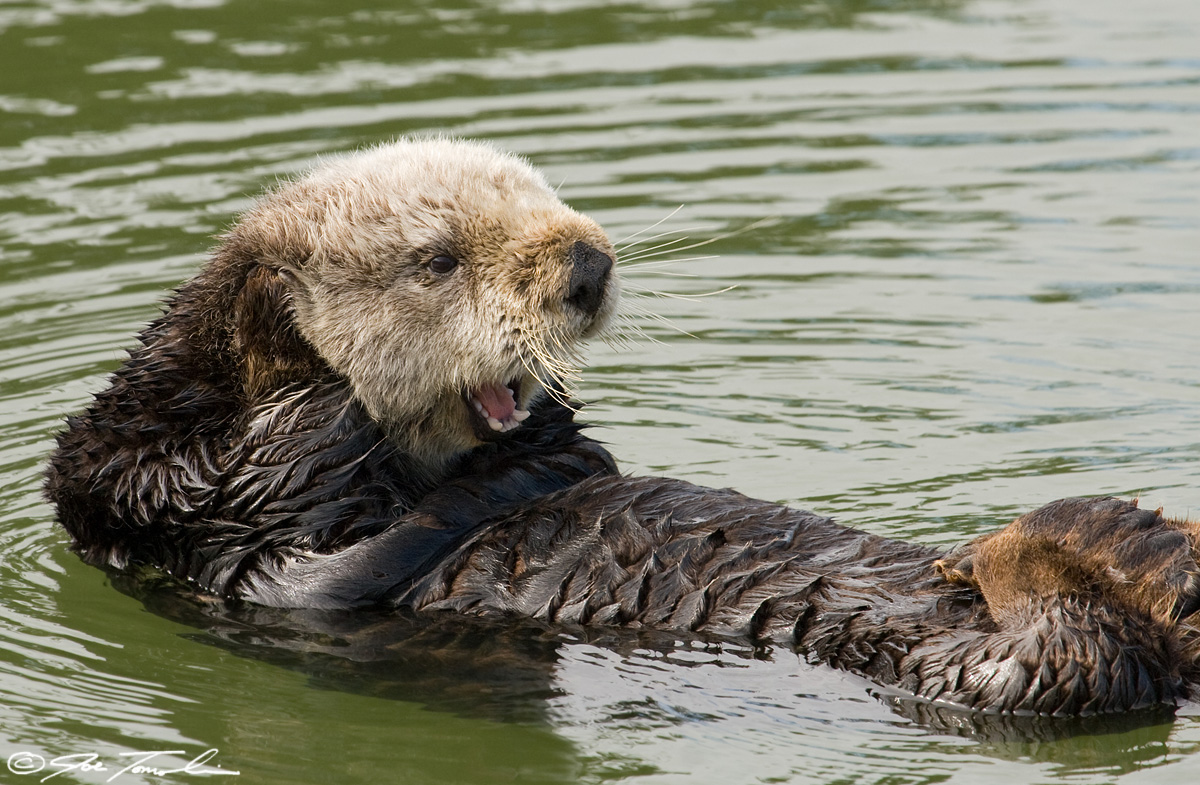
\includegraphics[
%width=\w, height=\h, 
%valign=t]{otter.jpg}
%\includegraphics[
%width=\w, height=\h, 
%valign=t]{kelp.jpg}
%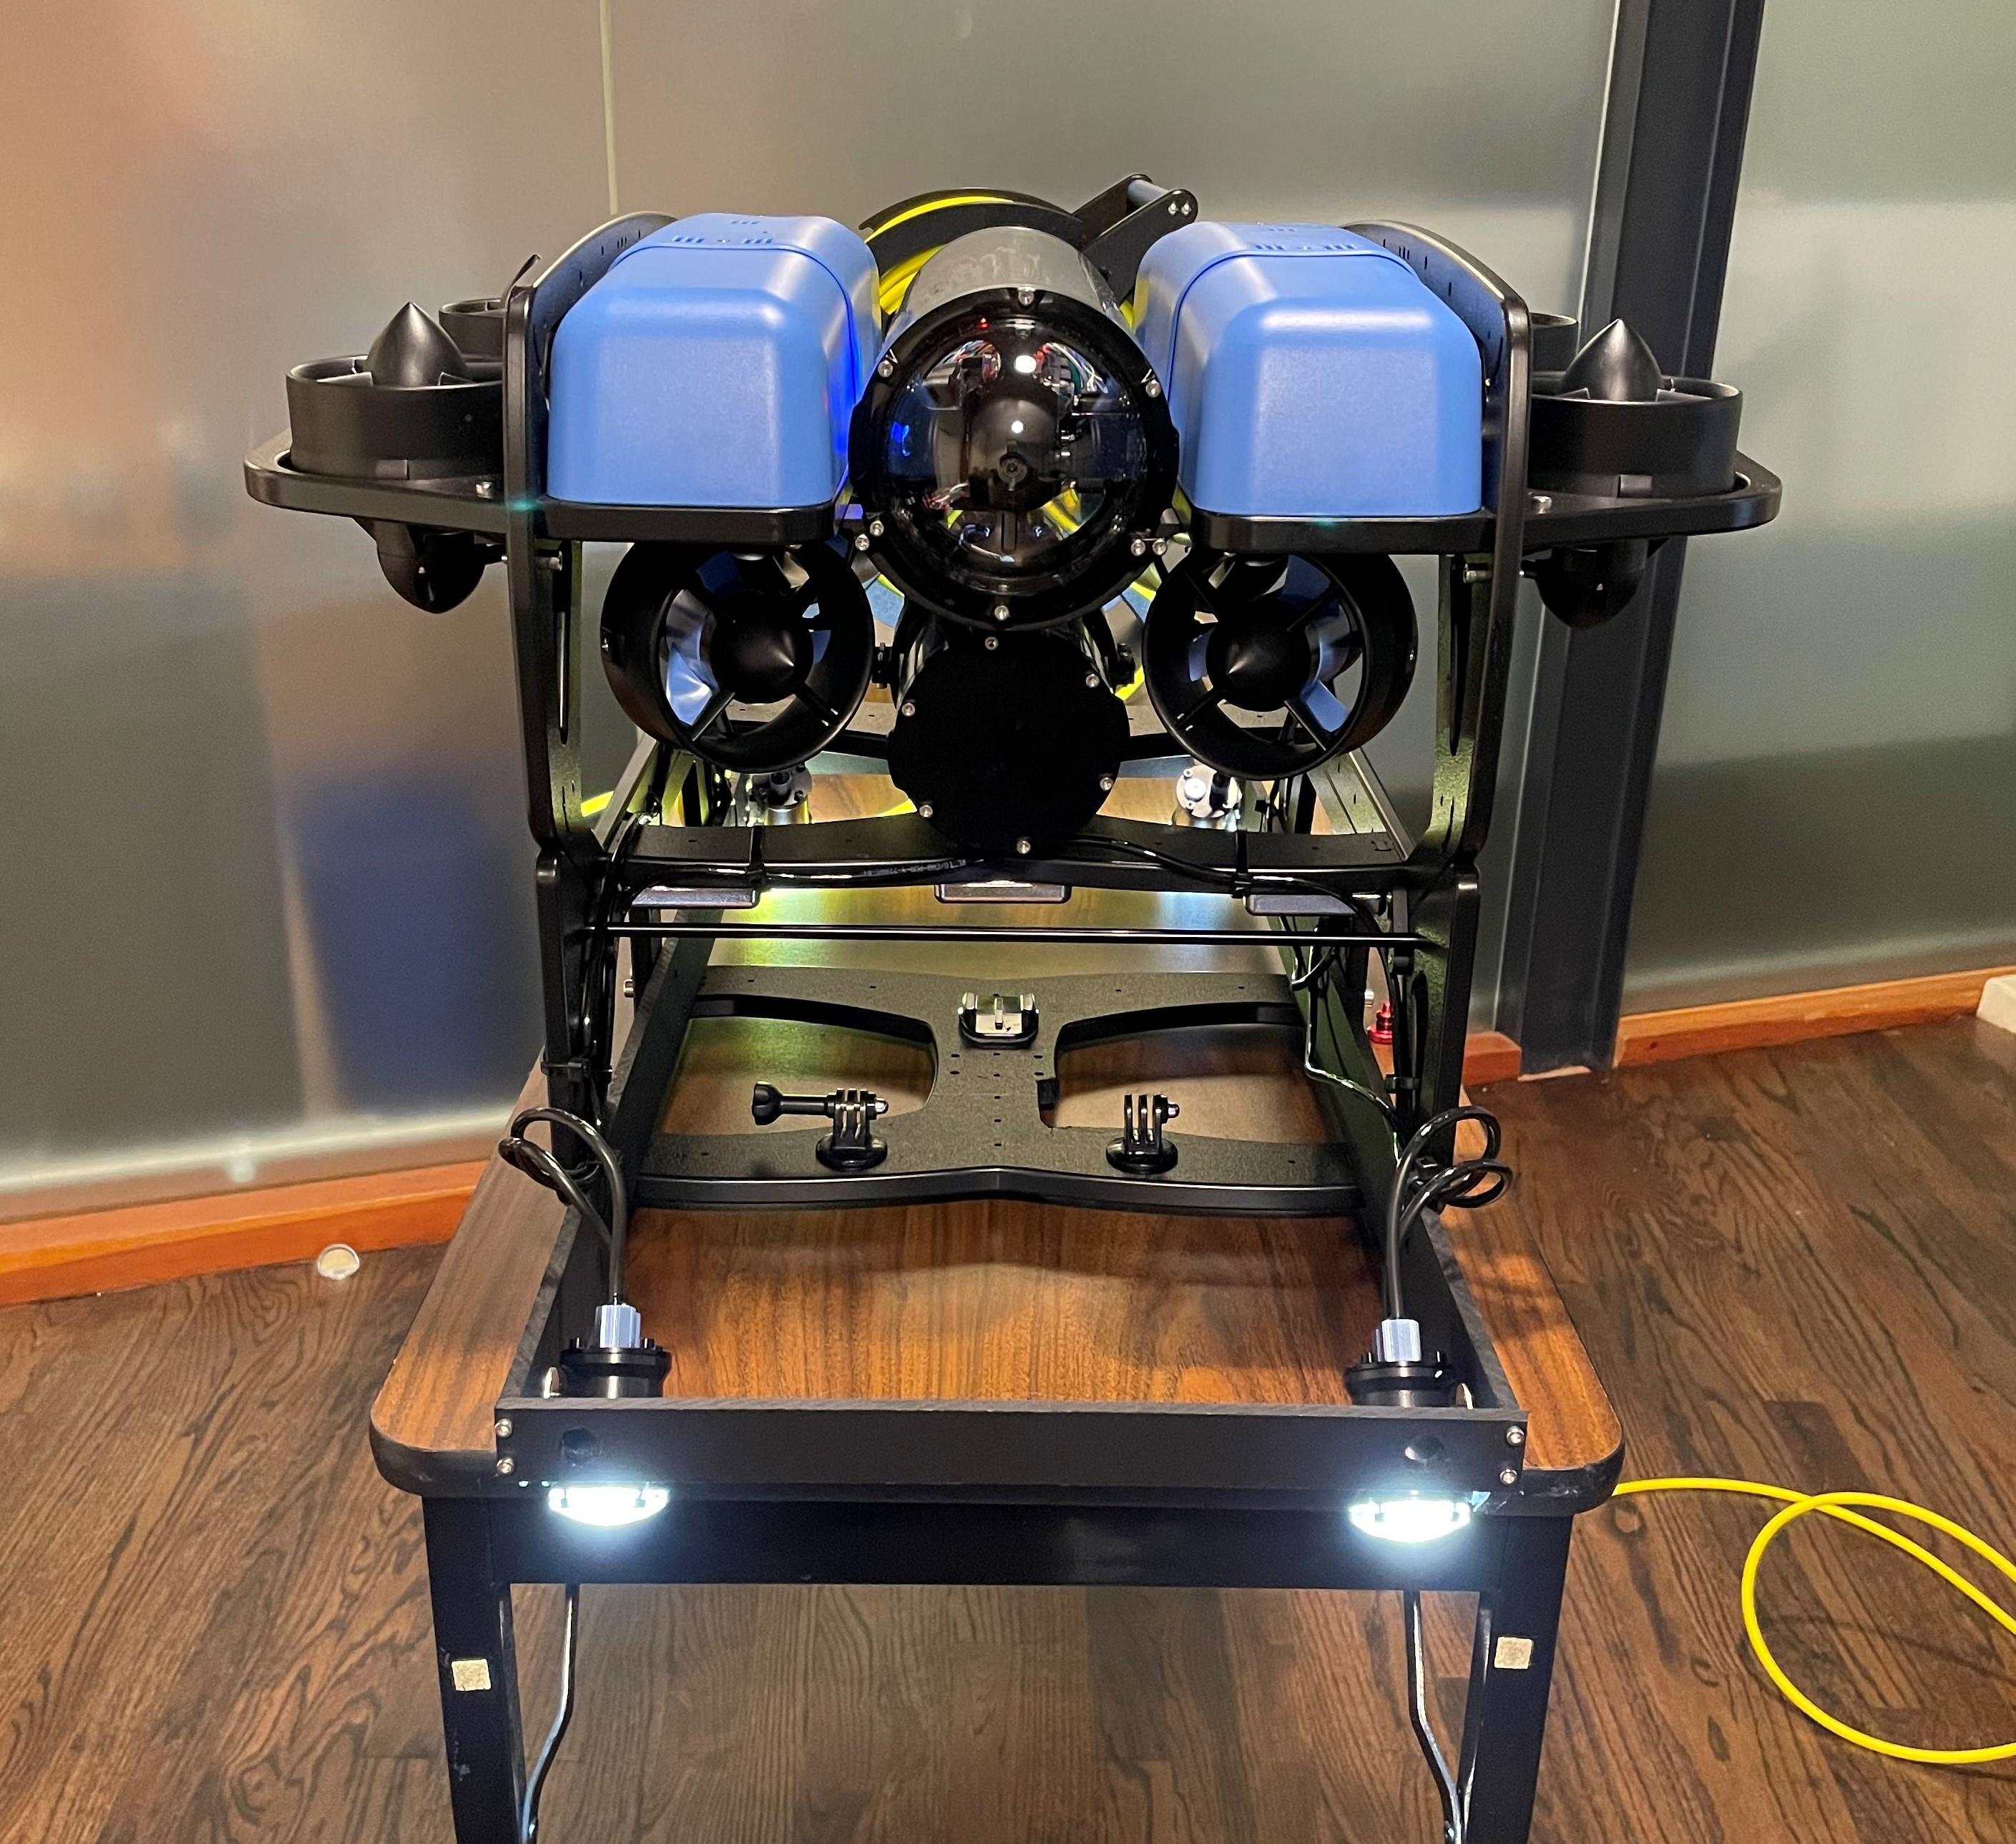
\includegraphics[
%width=\w, height=\h, 
%valign=t]{ROV.jpg}
%\\
%\label{fig:figurename}
%\end{figure}

\vspace{20pt}
\centering

\includegraphics[width=4.5cm]{Port_logo.png}
\hspace{20pt}

\includegraphics[width=3.5cm]{logo.jpg}
\\

%\large{Conservation Programs and Partnerships}
%\large{
%\textit{%\textbf{
%Climate Resilience $\vert$ 
%Sustainable Seas $\vert$ 
%Clean Waters
%}
%% END title page~~~~~~~~~~~~~~~~~~~~~~~~~~~~~~~~~~~~~~~~~~~~~~~~~~~~ %%
\end{titlepage}




%% section: Overview ~~~~~~~~~~~~~~~~~~~~~~~~~~~~~~~~~~~~~~~~~~~~~~~~ %%
\section{Overview}
\label{Overview}
%% Overview ~~~~~~~~~~~~~~~~~~~~~~~~~~~~~~~~~~~~~~~~~~~~~~~~~~~~~~~~~~~~
This report is partitioned into two primary halves, with the addition of introductory \textit{Overview} and a concluding \textit{Next-steps} sections. 
The first primary half, \textit{Field Work}, reports progress and lessons-learned from preliminary days in the field with Port of Seattle personnel, including site evaluations, canopy kelp-forest operations, ROV methodological experimentation, tests of the acoustic GPS, and problem-solving regarding an emergent leak within the ROV. 
The latter half, \textit{Analyses} deals with progress regarding data management and analysis, including the development of a complete analytical workflow for ROV telemetry and sensor files, video processing, and preliminary image annotation in CoralNet to calculate percent-coverage of species and habitat type.  
Thanks to funding from the Port of Seattle, on August $16th$ Megan 
Williams was brought onboard as a Research Technician for this project. 
She is providing instrumental support with regards to data management, 
video processing, statistical analyses, and fieldwork. 
Her funding is currently through the end of this year and we are 
actively seeking funds to keep her on.  
In sum, we are in a strong position to make a push in September to complete our summer surveys while bull kelp is still present, and we will continue to develop our analyses to next include preliminary maps of our ROV surveys.
%% END section: Overview ~~~~~~~~~~~~~~~~~~~~~~~~~~~~~~~~~~~~~~~~~~~~ %%




%% section: Motivation ~~~~~~~~~~~~~~~~~~~~~~~~~~~~~~~~~~~~~~~~~~~~~~ %%
\section{Field Work}
\label{Field Work}

\subsection{\textit{Overview of preliminary summer 2022 field days}}
Thanks to vessel support from Randy Edwards and other Port of Seattle personnel, we were out on the water August $8th$, $12th$, and $15th$. 
Our objectives were to 
(\textit{1}) develop site-familiarity of locations of interest to the 
Port, and
(\textit{2}) evaluate how to optimally structure ROV surveys given the configuration of Elliott Bay kelp beds.
We explored the riprap along the Elliott Bay Marina, the kelp forest to 
the west of Elliot Bay Marina, Smith Cove where rock were deployed for 
bull kelp restoration, and several sites along Centennial Park.
By August $15th$ we had developed our survey methods sufficiently that 
we completed six $100m$ transects at two sites offshore of Centennial Park. 
You can see video previews of these surveys from both the 
downward-facing (see 
\href{https://drive.google.com/file/d/1BKpNbOoVZD69AsEt5G7JsOrkMyZvgtjx/view?usp=sharing}{here}
 \& 
\href{https://drive.google.com/file/d/1J8xVqzrCSNAGh-g5ZEFoMboQgHW_H4rA/view?usp=sharing}{here})
 and forward-facing cameras (see 
 \href{https://drive.google.com/file/d/1RK28xmY8yo-FMqfbQtPPxmdujq9r2AEu/view?usp=sharing}{here}
 \& 
\href{https://drive.google.com/file/d/1OGcqmQaU9CvSFK4At0ju36zfMBRCUGUl/view?usp=sharing}{here}).

\subsection{\textit{Operating the ROV within canopy kelp forests}}
One of the foremost uncertainties regarding operating a ROV within 
canopy kelp forests is the potential for the ROV's tether to become 
entangled such that the ROV becomes immobilized.  
We are pleased to report that due to the relatively small size of the 
ROV, its high maneuverability, and a positively buoyant tether, we have 
developed a protocol for surveying into---and then successfully 
extricating the ROV out of---canopy kelp forests, without incurring serious entanglement.
This requires careful communication and coordination between the two ROV and tether operators. 
The protocol for ROV extraction from a kelp forest is as follows (and 
you can see video of this 
\href{https://drive.google.com/file/d/1qdtdPwB8RHkjL27RRzu95MTenNgszDAC/view?usp=sharing}{here}.):

\begin{enumerate}
\item
At the conclusion of, e.g., a 100m transect into a forest with thick 
canopy, pivot the ROV $180^\circ$, pan the built-in ROV camera upwards, 
partially ascend the ROV, and obtain a visual on the path of the tether 
back towards the vessel. 
\item
Carefully start to follow the tether back out of the bed. 
Maintain tight tether control by reeling up the slack as the ROV motors 
back towards the vessel. 
\item
The ROV operator will need to maneuver around, above, or under, e.g., 
bull kelp stipes or tangles of stipes and blades.
Thanks to the buoyant tether, these maneuvers are best conducted near the surface, and additional depth can be utilized when necessary (see the latter half of Fig.~$1$ for the depth profile while maneuvering out of a bed).
\item
In instances where the tether has been obstructed (but not wrapped) by, 
e.g., a large mass of bull kelp fronds, careful application of tension 
on both ends of the tether from (\textit{1}) the tether operator and (\textit{2}) the ROV by targeted thrust may pull the tether free. 
\end{enumerate} 

\subsection{\textit{Acoustic GPS system}}
These preliminary days with the Port enabled testing of our WaterLinked 
G2 Acoustic GPS system (see 
\href{https://waterlinked.github.io/underwater-gps/introduction/}{here} 
for details). 
This system operates with 
(\textit{1}) an acoustic transmitter attached to the ROV, 
(\textit{2}) an acoustic antenna deployed off of the vessel that 
receives communication from the acoustic transmitter, and 
(\textit{3}) a topside-hub on the vessel that obtains a GPS fix, is connected to the ROV's laptop, and integrates information from the acoustic system. 
When all three components are in place, we can record and export 
precise geospatial coordinates of the ROV's position underwater (see 
the \textit{lat} and \textit{lon} columns of 
\href{https://github.com/zhrandell/Seattle_Aquarium_ROV_telemetry_imagery_analysis/blob/15b0c253a3292df240f1559ae9e0f73d25d6be66/ROV_telemetry/Cleaned/2022-08-15_11-57-51.csv}{this}
 cleaned ROV telemetry file). 

There are seven channels corresponding to seven frequency bands for 
the acoustic transmitter and antenna (see 
\href{https://waterlinked.github.io/underwater-gps/gui/settings/}{here} 
for details).
We initially encountered acoustic interference along channels $1$ and 
$3$ (along the $31.25-62.5$ and $93.75-125.0$ $kHz$ bands, 
respectively), and eventually found that channel 5 ($156.25-187.5$ 
$kHz$) consistently worked. 
 
\subsection{\textit{ROV survey methodology development}}
Having developed the methods necessary to successfully operate within canopy forests, and with reliable ROV position information, we 
experimented with different modalities of benthic surveys and landed 
upon a protocol tailored to the Port of Seattle kelp beds. 
The kelp beds around Elliot Bay Marina and along Centennial park are 
narrow (down a depth gradient, perpendicular to shore) and long 
(parallel to shore). 
We found it works well to run the ROV ``down" a bed, i.e., parallel to 
shore and through the thick of the forest. 
Given the narrow nature of the beds (perpendicular to shore), we can 
complete transects 
(\textit{1}) within the bed along the inside-margin (shallow, 
relatively close to shore), 
(\textit{2}) down the middle of the bed, 
(\textit{3}) within the bed along the outer-margin (deeper, relatively 
distanced from shore), and 
(\textit{4}) just outside the bed.
As the acoustic GPS has a $100m$ range, and as we have a $150m$ tether, 
we are successfully able to conduct $100m$ transects.  
Depending upon current and how hard the ROV motors need to work, we can 
complete three or four transects on a single battery of the ROV (we 
have three ROV batteries).

\subsection{\textit{ROV leak}}
The ROV presented a leak at the end of August that necessitated rescheduling a couple days in the field with Port. 
Identifying the source of this leak has been a process of trial-and-error, and we have tackled multiple potential fail points: (\textit{1}) we replaced the acrylic housing for the electronics compartment as there were small scratches running across the double O-ring seal, and (\textit{2}) we replaced all the O-rings in the ROV. 
On August $7th$ we definitively identified a failed power cable as the source of a small leak, and a new cable has been ordered---as have numerous spare parts---to ensure future leaks do not delay operations. 
Furthermore, we are exploring the idea of purchasing a second ROV with 
a complete set of hardware, such that if one ROV goes down, the second 
can be seamlessly rotated into the field. 
%% END section: Field Work ~~~~~~~~~~~~~~~~~~~~~~~~~~~~~~~~~~~~~~~~~~ %%





%% section: Methods ~~~~~~~~~~~~~~~~~~~~~~~~~~~~~~~~~~~~~~~~~~~~~~ %%
\section{Video and data management and analyses}
\label{Analyses}

\subsection{\textit{Analytical workflow development}}
We have developed an overarching workflow and the associated details for the precise steps and code necessary to perform a 
variety of functions related to file management for the ROV telemetry 
files and $4K$ $30fps$ video and extracted stills. 
All required steps are codified in our \textit{Overarching\_Workflow} 
document (linked \href{https://github.com/zhrandell/Seattle_Aquarium_ROV_telemetry_imagery_analysis/blob/main/documents/Overarching_Workflow.xlsx}{here}; click either the ``view raw" or ``download" button),
 as is a tracklog to monitor file status. 
This document also lays out file naming conventions, file paths, links to requisite open-source code, etc. 
The steps are grouped as follows:

\begin{enumerate}[label=\textbf{\Alph*}:]
\item 
Configure a local machine to access open-source CCR 
files, conduct analyses, and push edits to GitHub repository.
\item 
Extract, save, and backup ROV telemetry (.csv) and Ping Sonar 
Alitimeter (.bin) files and benthic- and forward-facing GoPro video 
(.mp4). 
\item
Work with and merge the .csv and .bin files to 
generate a dive log at the $1s$ scale, i.e. with one second intervals 
(rows), including latitude and longitude, distance traveled between 
coordinates, ROV altitude above the seafloor, depth, temperature, etc.
\item
Video processing such as clipping the .mp4 videos to the precise survey
transects, color-matching (if needed), and extracting and saving stills 
from video.
\item 
File management to save and back-up cleaned/processed video and stills 
and eventually delete older file versions. 
\item Upload image stills to CoralNet, annotate imagery 
with percent-cover categories, review and correct (if necessary) 
algorithm predictions, save and download the .csv CoralNet file.
 \item 
Merge the CoralNet .csv containing species and habitat data 
with the merged ROV telemetry .csv file to produce a final combined ROV 
telemetry plus community and habitat data. 
\end{enumerate}

\subsection{\textit{Mapping Station at the Seattle Aquarium}}
We are working with the Seattle Aquarium's IT department to develop a 
custom \textit{Mapping Station} at the Market Square building. 
This will include a computer optimized for processing speed, memory, 
and intensive video/analytical tasks such as the compilation of 
Artificial Intelligence (AI) algorithms and processing of $4K$ 
imagery on $4K$ computer screens. 

This \textit{Mapping Station} will provide an onsite base for our 
project, and in addition to using it ourselves, we envision it will 
provide an interface for volunteers and also Port of Seattle personnel 
or associates that want to become familiar with video processing, 
AI analyses, mapping, etc. 
We look forward to opportunities to share our code, video processing 
approach, AI methods, and spatial analyses in-person with interested 
parties.

\subsection{\textit{Open-source resource development}}
We are striving to maintain transparency and accessibility throughout 
this project, both with regards to hardware such as our customized ROV, as well as software, including maintaining a record of code, changes made to code, and the use of open-source programs where possible.
We currently have two public repositories on GitHub: 

\begin{itemize}
\item 
\href{https://github.com/zhrandell/Seattle_Aquarium_ROV_development}{Seattle$\_$Aquarium$\_$ROV$\_$development}
contains general information that may be of interest to collaborators 
or members of the public.  
It provides a broad overview of our project including links to summary 
documents, articles and interviews, information about the ROV and links 
to its components, and links to photos and video from the ROV. 
\item
\href{https://github.com/zhrandell/Seattle_Aquarium_ROV_telemetry_imagery_analysis}{Seattle$\_$Aquarium$\_$ROV$\_$telemetry$\_$imagery$\_$analysis}
is more in the weeds, and contains code to convert and manage files, 
extract stills from video, create figures, as well as links to coding 
and analytical resources. 
As it is public, interested parties can clone (i.e., download) this 
repository to their local machine in order to conduct the same 
analyses, file conversions, and data management, assuming they have the 
required programs (linked 
\href{https://github.com/zhrandell/Seattle_Aquarium_ROV_development/blob/main/documents/hardware_software.md#rov-firmware-flight-programs--analytical-software}{here})
 installed.  
\end{itemize}

\subsection{\textit{Video processing}}
The only program we are currently using that is not freely open-source 
is 
\href{https://www.cyberlink.com/products/powerdirector-video-editing-software/features_en_US.html?r=1}{Cyberlink
 PowerDirector}, a subscription based video editing program.
With this program we can trim files down to specific survey transects, 
as well as color match to correct any instances in which the white 
balance deviates.

Furthermore, we now have Python
\href{https://github.com/zhrandell/Seattle_Aquarium_ROV_telemetry_imagery_analysis/blob/main/code/4k_to_still.py}{code} in place to extract stills from the $4K$ $30fps$ GoPro video. 
As we can easily control the interval at which stills are extracted 
(e.g., take a still every $5$, $10$, or $20$ seconds), we can ensure 
that for any given ROV dive, our stills do not overlap one another 
(i.e., double-count), nor do they miss information in-between stills 
(i.e., under-count).   

\subsection{\textit{Telemetry files}}
We have developed the steps and code to work with and manage 
(\textit{1}) the .csv telemetry file containing a record of the ROV's 
dive, including latitude/longitude information, and the (\textit{2}) 
Ping Sonar Altimeter .bin file, containing a record of the ROV's height 
above the seafloor. 
The telemetry file required extensive pruning, code for which you can 
find 
\href{https://github.com/zhrandell/Seattle_Aquarium_ROV_telemetry_imagery_analysis/blob/main/code/tracklog_cleaning.R}{here}.
The .bin Ping file required conversion from .bin to .csv (code 
\href{https://github.com/zhrandell/Seattle_Aquarium_ROV_telemetry_imagery_analysis/blob/main/code/Ping_to_csv.py}{here}).
The Ping data required a bit of massaging (e.g., 
\href{https://github.com/zhrandell/Seattle_Aquarium_ROV_telemetry_imagery_analysis/issues/3#issuecomment-1225997792}{here})
 as it samples many times per second and we needed to merge it with the 
 ROV telemetry file which is at the $1s$ scale.
You can see code for merging these files  
\href{https://github.com/zhrandell/Seattle_Aquarium_ROV_telemetry_imagery_analysis/blob/main/code/ROV_telemetry_file_work.R}{here}.

\begin{figure}[h!]
\centering
\subfloat[]{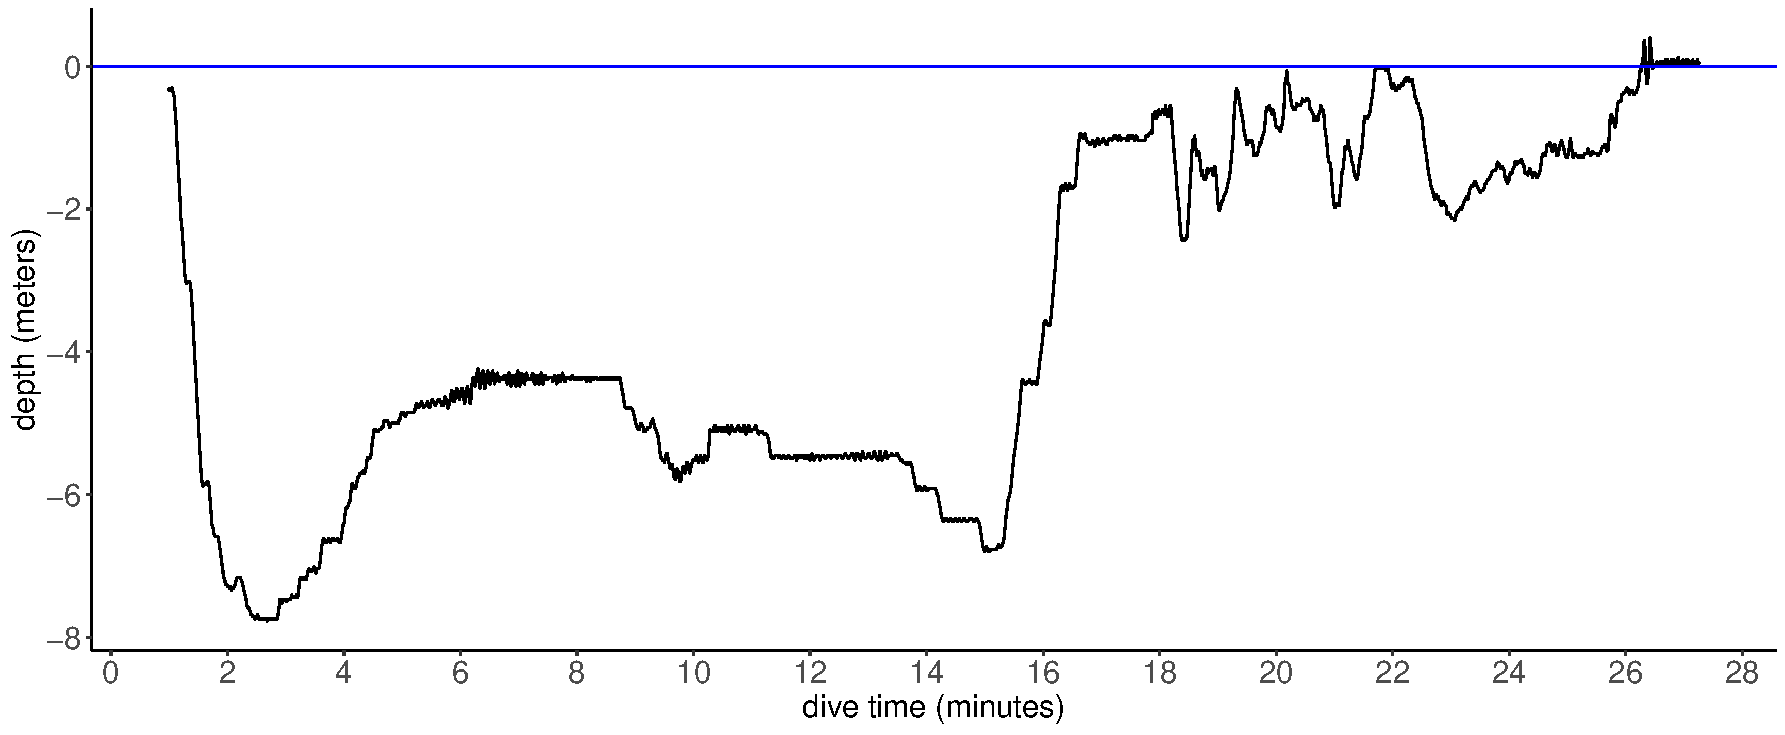
\includegraphics[
width=12cm, height=5cm]{divelog.pdf}}
\caption{
(a) the depth log of one of the August $15th$ surveys, with 
the first half recording a profile of a survey, and the latter half 
recording depth while navigating out of a kelp bed. 
}
\label{divelog}
\end{figure}

You can see an example of a completely cleaned and processed ROV 
telemetry file 
\href{https://github.com/zhrandell/Seattle_Aquarium_ROV_telemetry_imagery_analysis/blob/main/ROV_telemetry/Cleaned/2022-08-15_09-57-40.csv}{here}
 with columns such as time in $hh:mm:ss$ (\textit{time}), 
a running tally of the ROV's flight time (\textit{flight$\_$time}), 
depth, 
compass heading (\textit{heading}), 
\textit{battery$\_$remaining}, and 
geospatial information such as 
latitude (\textit{lat}),
longitude (\textit{lon}),
and the distance in meters between each GPS point (\textit{EucDIS}). 
The last two columns contain information from the Ping Sonar 
Altimeter such as the ROV's distance above the 
seafloor (\textit{avg$\_$dist}) and percent-confidence 
(\textit{avg$\_$conf}). 

\subsection{\textit{Preliminary CoralNet analyses}}
We used the open-source AI web interface CoralNet to create a project, upload percent-cover categories, and annotate a preliminary set of images (Fig.~$2$). 
You can review the list of percent-coverage categories for species as well as habitat type 
\href{https://github.com/zhrandell/Seattle_Aquarium_ROV_telemetry_imagery_analysis/blob/main/documents/CoralNet_Percent_Cover_Classifications.xlsx}{here} (click either the ``view raw" or ``download" button).
Once these categories were entered into CoralNet, we uploaded extracted stills from our $4K$ video from offshore of Centennial Park, and conducted a preliminary proof-of-concept series of annotations.
Once the annotations were complete, we exported the resulting .csv files, and merged them with the relevant rows from the ROV telemetry file. 
What you see 
\href{https://github.com/zhrandell/Seattle_Aquarium_ROV_telemetry_imagery_analysis/blob/15b0c253a3292df240f1559ae9e0f73d25d6be66/ROV_telemetry/Cleaned/Telemetry_and_CoralNet.xlsx}{here} (click either the ``view raw" or ``download" button)
 is the final product of our analytical workflow chain of events, i.e., the complete record of our dive including depth, latitude/longitude, Ping Altimeter data, as well as the corresponding community structure identified at those precise seconds throughout the dive.  

\begin{figure}[h!]
\centering
\subfloat[]{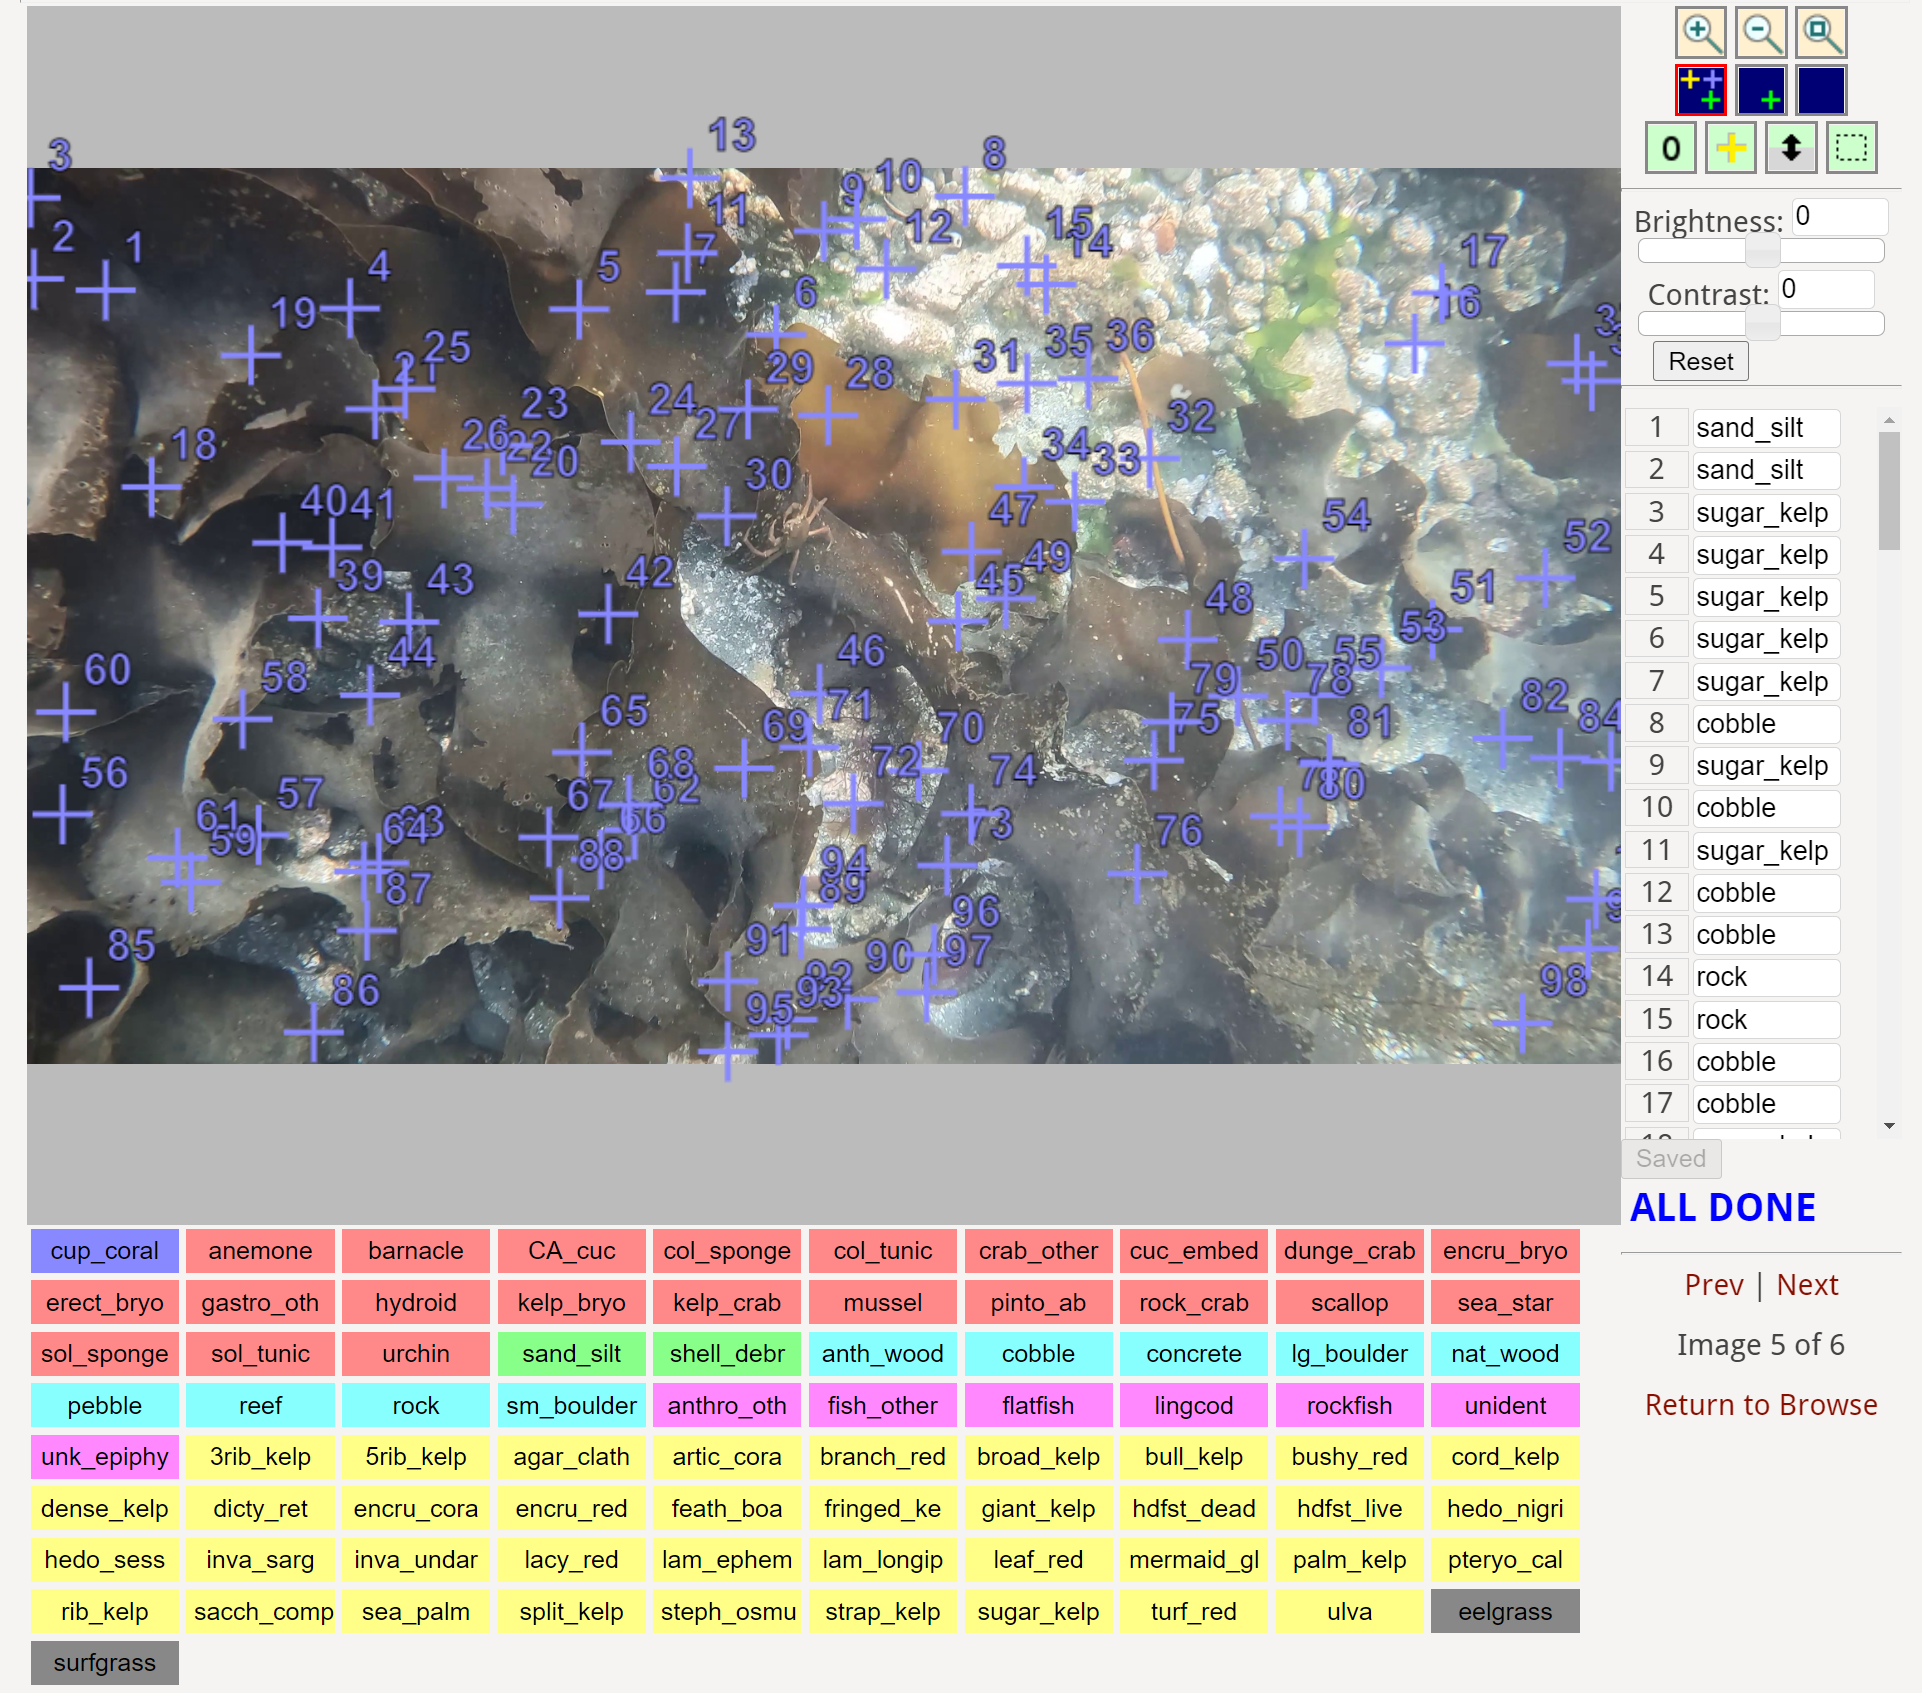
\includegraphics[
width=\w, height=\h, valign=t]{CoralNet_1.png}}
\subfloat[]{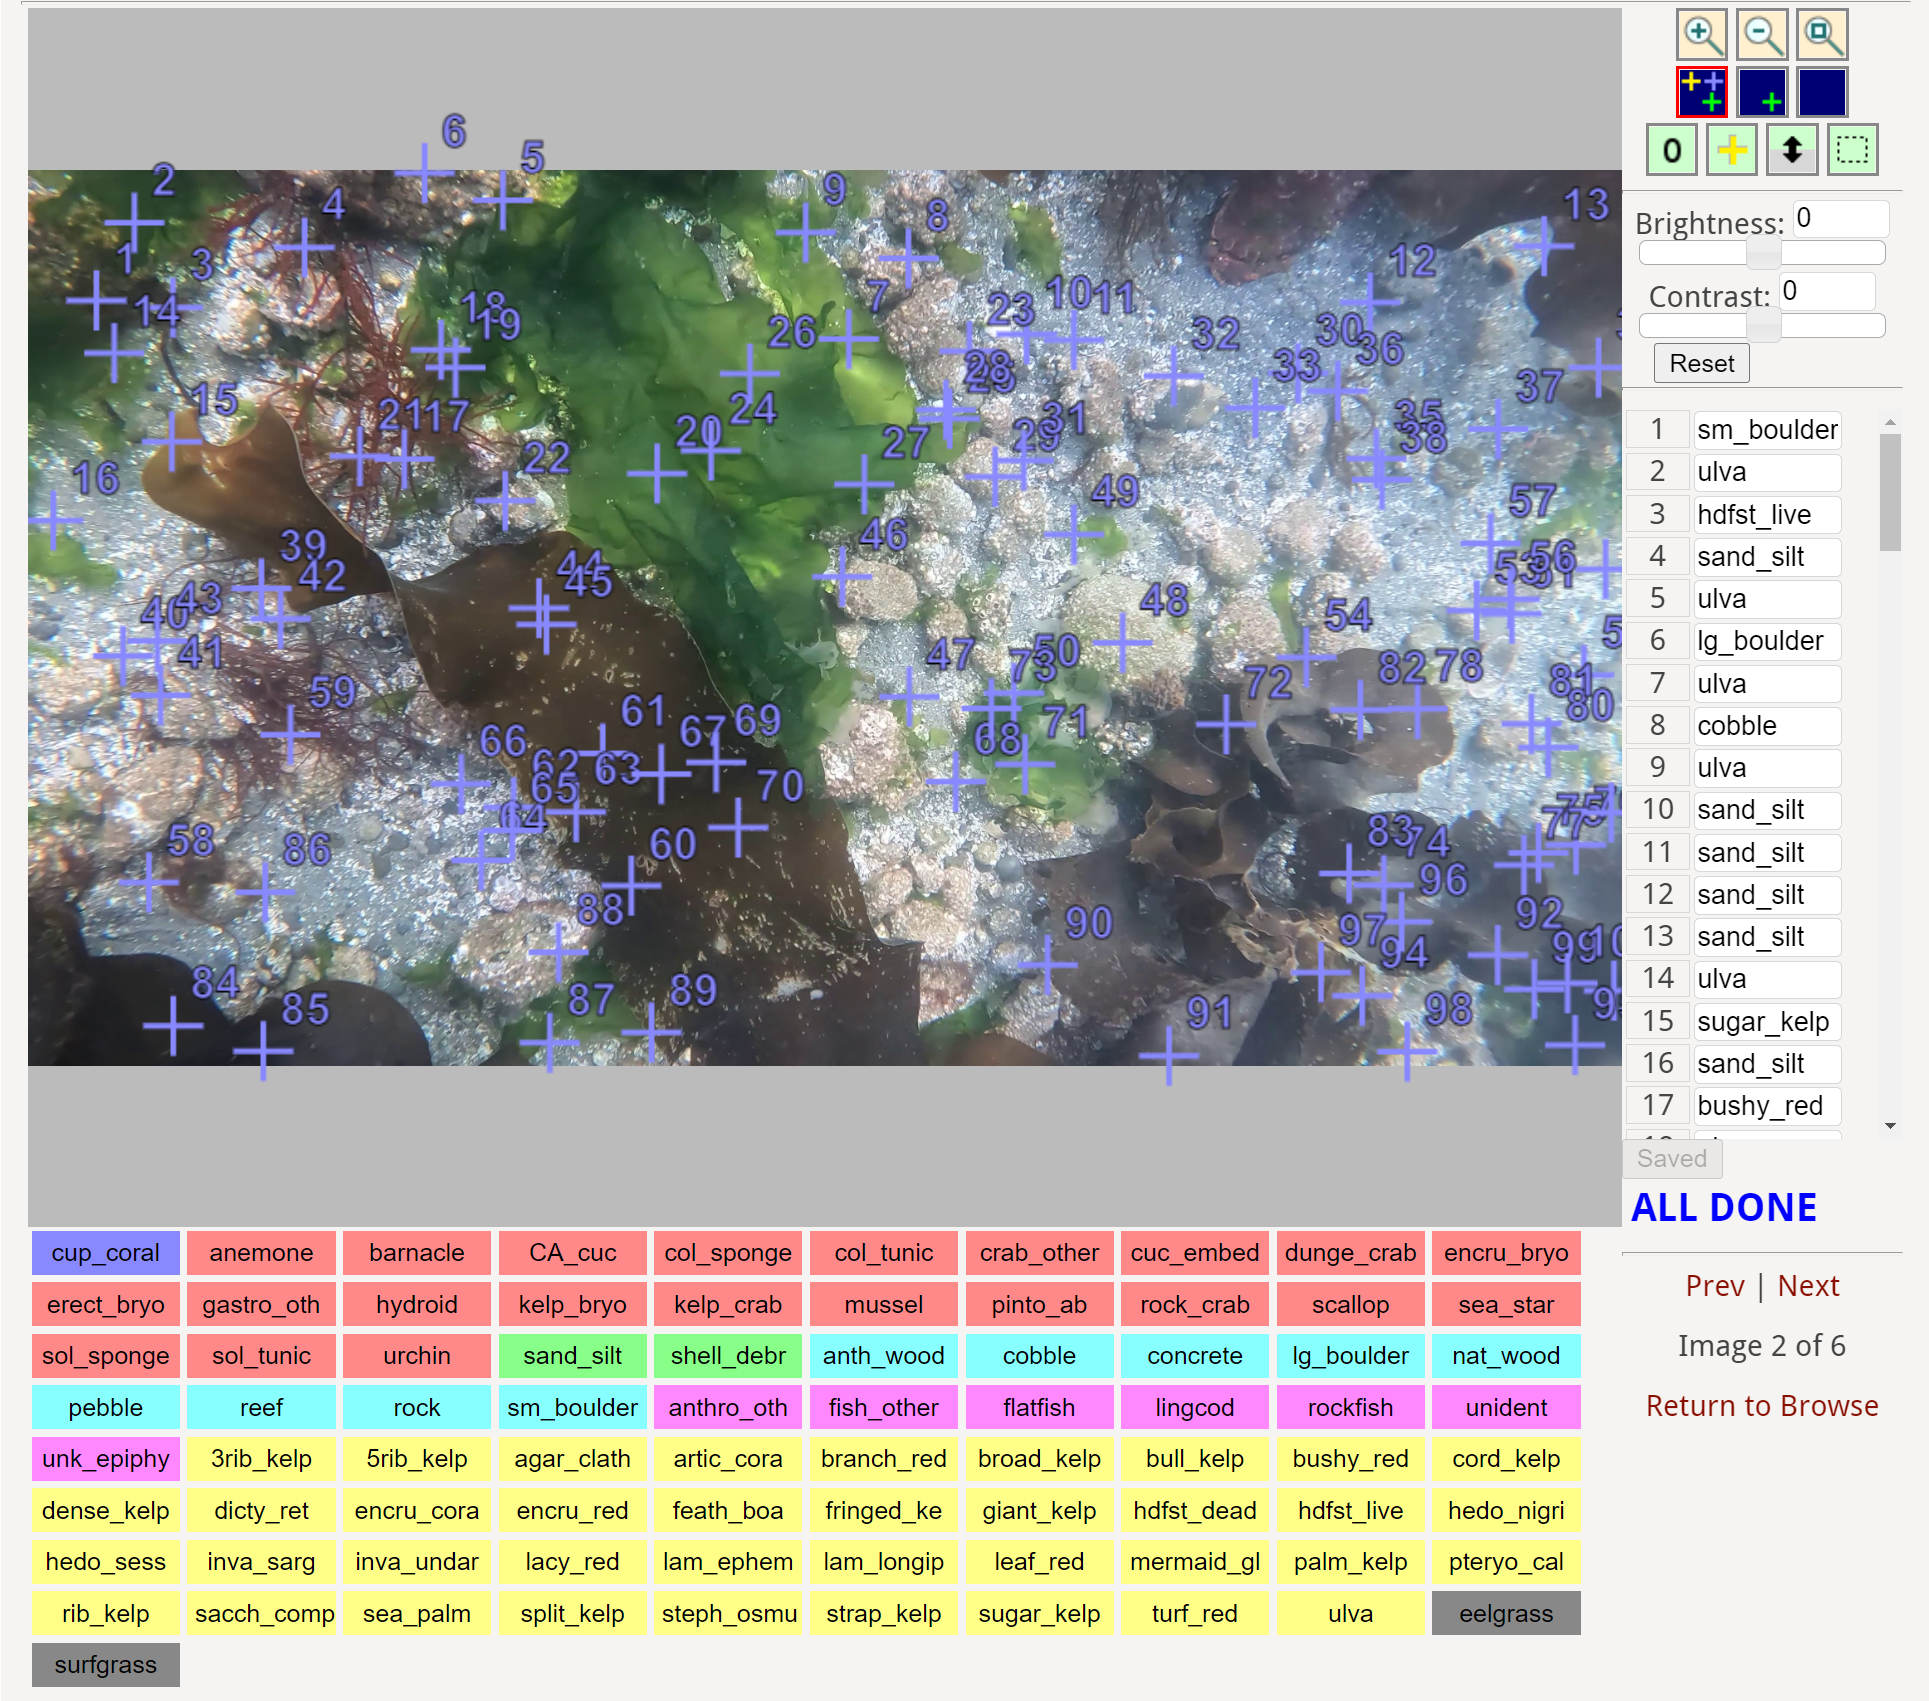
\includegraphics[
width=\w, height=\h, valign=t]{CoralNet_2.png}}
\caption{
(a) \& (b) two different stills extracted from $4K$ $30fps$ GoPro video 
uploaded and annotated within Coral to calculate percent coverage of 
various species as well as substrate type.
}
\label{CoralNet_pics}
\end{figure}
%% END section: Analyses ~~~~~~~~~~~~~~~~~~~~~~~~~~~~~~~~~~~~~~~~~~~ %%



%% brief wrap-up section ~~~~~~~~~~~~~~~~~~~~~~~~~~~~~~~~~~~~~~~~~~~~ %%
\section{Next-steps}
Our next-steps in the field include a flurry of surveys in September to 
finish our summer 2022 work in Elliot Bay, along Centennial Park, and in
the East and West Waterways. 
On the analytical side, having developed our analytical workflow, we 
will enact it through processing full-length ROV dives, as well as initiate community/habitat data visualization. 
We will also simultaneously push to develop the mapping portion of this 
project through using the latitude/longitude coordinates recorded by our GPS system. 
In short, we are on track and we look forward to advancing this project with Port personnel.  
%% END brief wrap-up section ~~~~~~~~~~~~~~~~~~~~~~~~~~~~~~~~~~~~~~~~ %%



%% section: References ~~~~~~~~~~~~~~~~~~~~~~~~~~~~~~~~~~~~~~~~~~~~~~ %%
%\clearpage
%\section{References}
%\printbibliography[heading=none]
%\label{References}
%% END section: References ~~~~~~~~~~~~~~~~~~~~~~~~~~~~~~~~~~~~~~~~~~ %%


%% END document ~~~~~~~~~~~~~~~~~~~~~~~~~~~~~~~~~~~~~~~~~~~~~~~~~~~~~ %%
\end{document}
%% END document ~~~~~~~~~~~~~~~~~~~~~~~~~~~~~~~~~~~~~~~~~~~~~~~~~~~~~ %%































